\chapter{Implementacija i korisničko sučelje}
		
		\section{Korištene tehnologije i alati}
		
			 
			 Za izradu projekta koristili smo različite tehnologije, alate i platforme kako bismo učinkovito surađivali i razvili visokokvalitetnu aplikaciju. Za međusobnu komunikaciju unutar tima koristili smo aplikacije WhatsApp\footnote{\url{https://www.whatsapp.com/}} i Discord\footnote{\url{https://discord.com/}} što nam je omogućilo brz i jednostavan način dijeljenja informacija i dogovaranja.
			 
			 Sustav za upravljanje izvornim kodom bio je Git\footnote{\url{https://git-scm.com/}}, a repozitorij projekta smješten je na web platformi GitHub\footnote{\url{https://github.com/}}. Ovo nam je omogućilo sinkronizaciju rada, praćenje promjena i suradnju na kodu na učinkovit način. Za izradu UML dijagrama korišten je alat Astah UML\footnote{\url{https://astah.net/products/astah-uml/}}, pružajući jasnu vizualizaciju strukture i odnosa unutar projekta.
			 
			 Integrirano razvojno okruženje (IDE) koje smo koristili bilo je IntelliJ\footnote{\url{https://www.jetbrains.com/idea/}}, razvijeno u tvrtki JetBrains. IntelliJ je posebno prilagođen za rad s računalnim softverom napisanim u Javi, Kotlinu i Groovyju te pruža potporu za druge popularne jezike kao što su Python, JavaScript i TypeScript. To osigurava dosljedno iskustvo rada na različitim operativnim sustavima - Windows, macOS i Linux.
			 
			 Za backend aplikacije koristili smo Spring Boot\footnote{\url{https://spring.io/projects/spring-boot/}}, radni okvir baziran na Javi koji nudi autokonfiguraciju za olakšavanje početka razvoja, ali istovremeno omogućuje programerima da prilagode konfiguraciju prema potrebama.
			 
			 Frontend je implementiran pomoću Reacta\footnote{\url{https://react.dev/}}, biblioteke u JavaScriptu\footnote{\url{https://www.javascript.com/}} za izgradnju korisničkih sučelja. React se temelji na komponentama što je omogućilo razvoj složenih aplikacija s jasnom strukturom.\\
			 
			 Baza podataka projekta bila je PostgreSQL\footnote{\url{https://www.postgresql.org/}}, otvoreni sustav za upravljanje relacijskom bazom podataka. Konačno, aplikacija se nalazi na Renderu\footnote{\url{https://render.com/}}, oblak platformi kao usluzi, koja podržava različite programske jezike i omogućuje laku implementaciju i upravljanje modernim aplikacijama.
			 
			 Za ispitivanje sustava korišten je radni okvir Selenium\footnote{\url{https://www.seleniumhq.org/}} koji pruža automatsko testiranje kako bi se osigurala funkcionalnost i stabilnost sustava.
			 
			 Kombinacija ovih tehnologija i alata omogućila je timu učinkovit rad i uspješan razvoj aplikacije.
			
			
			\eject 
		
	
		\section{Ispitivanje programskog rješenja}
			
			\textbf{\textit{dio 2. revizije}}\\
			
			 \textit{U ovom poglavlju je potrebno opisati provedbu ispitivanja implementiranih funkcionalnosti na razini komponenti i na razini cijelog sustava s prikazom odabranih ispitnih slučajeva. Studenti trebaju ispitati temeljnu funkcionalnost i rubne uvjete.}
	
			
			\subsection{Ispitivanje komponenti}
			\textit{Potrebno je provesti ispitivanje jedinica (engl. unit testing) nad razredima koji implementiraju temeljne funkcionalnosti. Razraditi \textbf{minimalno 6 ispitnih slučajeva} u kojima će se ispitati redovni slučajevi, rubni uvjeti te izazivanje pogreške (engl. exception throwing). Poželjno je stvoriti i ispitni slučaj koji koristi funkcionalnosti koje nisu implementirane. Potrebno je priložiti izvorni kôd svih ispitnih slučajeva te prikaz rezultata izvođenja ispita u razvojnom okruženju (prolaz/pad ispita). }
			
			
			
			\subsection{Ispitivanje sustava}
			
			 \textit{Potrebno je provesti i opisati ispitivanje sustava koristeći radni okvir Selenium\footnote{\url{https://www.seleniumhq.org/}}. Razraditi \textbf{minimalno 4 ispitna slučaja} u kojima će se ispitati redovni slučajevi, rubni uvjeti te poziv funkcionalnosti koja nije implementirana/izaziva pogrešku kako bi se vidjelo na koji način sustav reagira kada nešto nije u potpunosti ostvareno. Ispitni slučaj se treba sastojati od ulaza (npr. korisničko ime i lozinka), očekivanog izlaza ili rezultata, koraka ispitivanja i dobivenog izlaza ili rezultata.\\ }
			 
			 \textit{Izradu ispitnih slučajeva pomoću radnog okvira Selenium moguće je provesti pomoću jednog od sljedeća dva alata:}
			 \begin{itemize}
			 	\item \textit{dodatak za preglednik \textbf{Selenium IDE} - snimanje korisnikovih akcija radi automatskog ponavljanja ispita	}
			 	\item \textit{\textbf{Selenium WebDriver} - podrška za pisanje ispita u jezicima Java, C\#, PHP koristeći posebno programsko sučelje.}
			 \end{itemize}
		 	\textit{Detalji o korištenju alata Selenium bit će prikazani na posebnom predavanju tijekom semestra.}
			
			\eject 
		
		
		\section{Dijagram razmještaja}
			
			Dijagram razmještaja~\ref{fig:dijagramRazmjestaja} opisuje topologiju sklopovlja i programsku potporu koja se koristi u implementaciji sustava u njegovom radnom okruženju. Sustav je baziran na arhitekturi "klijent-poslužitelj". Poslužiteljsko računalo (Render) sadrži web poslužitelj na kojem se nalazi naša web aplikacija te sadrži poslužitelj baze podataka na kojemu je naša Postgres baza podataka. Komunikacija između klijenta i poslužitelja obavlja se preko sigurnog kanala ostvarenog protokolom HTTPS.
			
			
			 \begin{figure}[H]
				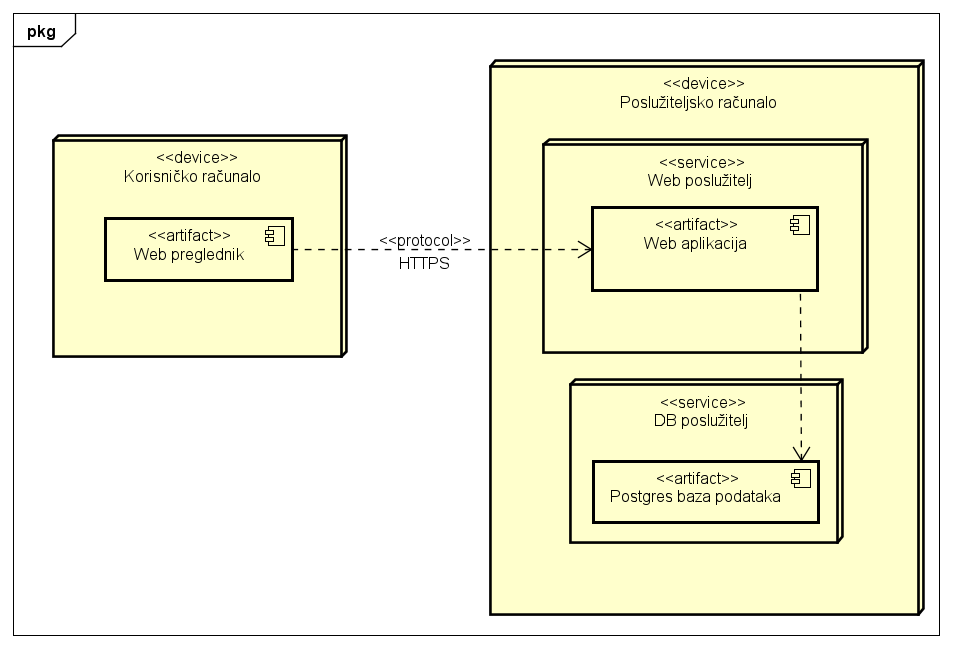
\includegraphics[width=\textwidth]{slike/dijagramRazmjestaja.PNG} %veličina u odnosu na širinu linije
				\caption{Dijagram razmještaja}
				\label{fig:dijagramRazmjestaja} %label mora biti drugaciji za svaku sliku
			\end{figure}
			
			
			\eject 
		
		\section{Upute za puštanje u pogon}
		
			\textbf{\textit{dio 2. revizije}}\\
		
			 \textit{U ovom poglavlju potrebno je dati upute za puštanje u pogon (engl. deployment) ostvarene aplikacije. Na primjer, za web aplikacije, opisati postupak kojim se od izvornog kôda dolazi do potpuno postavljene baze podataka i poslužitelja koji odgovara na upite korisnika. Za mobilnu aplikaciju, postupak kojim se aplikacija izgradi, te postavi na neku od trgovina. Za stolnu (engl. desktop) aplikaciju, postupak kojim se aplikacija instalira na računalo. Ukoliko mobilne i stolne aplikacije komuniciraju s poslužiteljem i/ili bazom podataka, opisati i postupak njihovog postavljanja. Pri izradi uputa preporučuje se \textbf{naglasiti korake instalacije uporabom natuknica} te koristiti što je više moguće \textbf{slike ekrana} (engl. screenshots) kako bi upute bile jasne i jednostavne za slijediti.}
			
			
			 \textit{Dovršenu aplikaciju potrebno je pokrenuti na javno dostupnom poslužitelju. Studentima se preporuča korištenje neke od sljedećih besplatnih usluga: \href{https://aws.amazon.com/}{Amazon AWS}, \href{https://azure.microsoft.com/en-us/}{Microsoft Azure} ili \href{https://www.heroku.com/}{Heroku}. Mobilne aplikacije trebaju biti objavljene na F-Droid, Google Play ili Amazon App trgovini.}
			
			
			\eject 